\documentclass[twoside]{book}

% Packages required by doxygen
\usepackage{fixltx2e}
\usepackage{calc}
\usepackage{doxygen}
\usepackage[export]{adjustbox} % also loads graphicx
\usepackage{graphicx}
\usepackage[utf8]{inputenc}
\usepackage{makeidx}
\usepackage{multicol}
\usepackage{multirow}
\PassOptionsToPackage{warn}{textcomp}
\usepackage{textcomp}
\usepackage[nointegrals]{wasysym}
\usepackage[table]{xcolor}

% NLS support packages
\usepackage[french]{babel}

% Font selection
\usepackage[T1]{fontenc}
\usepackage[scaled=.90]{helvet}
\usepackage{courier}
\usepackage{amssymb}
\usepackage{sectsty}
\renewcommand{\familydefault}{\sfdefault}
\allsectionsfont{%
  \fontseries{bc}\selectfont%
  \color{darkgray}%
}
\renewcommand{\DoxyLabelFont}{%
  \fontseries{bc}\selectfont%
  \color{darkgray}%
}
\newcommand{\+}{\discretionary{\mbox{\scriptsize$\hookleftarrow$}}{}{}}

% Page & text layout
\usepackage{geometry}
\geometry{%
  a4paper,%
  top=2.5cm,%
  bottom=2.5cm,%
  left=2.5cm,%
  right=2.5cm%
}
\tolerance=750
\hfuzz=15pt
\hbadness=750
\setlength{\emergencystretch}{15pt}
\setlength{\parindent}{0cm}
\setlength{\parskip}{0.2cm}
\makeatletter
\renewcommand{\paragraph}{%
  \@startsection{paragraph}{4}{0ex}{-1.0ex}{1.0ex}{%
    \normalfont\normalsize\bfseries\SS@parafont%
  }%
}
\renewcommand{\subparagraph}{%
  \@startsection{subparagraph}{5}{0ex}{-1.0ex}{1.0ex}{%
    \normalfont\normalsize\bfseries\SS@subparafont%
  }%
}
\makeatother

% Headers & footers
\usepackage{fancyhdr}
\pagestyle{fancyplain}
\fancyhead[LE]{\fancyplain{}{\bfseries\thepage}}
\fancyhead[CE]{\fancyplain{}{}}
\fancyhead[RE]{\fancyplain{}{\bfseries\leftmark}}
\fancyhead[LO]{\fancyplain{}{\bfseries\rightmark}}
\fancyhead[CO]{\fancyplain{}{}}
\fancyhead[RO]{\fancyplain{}{\bfseries\thepage}}
\fancyfoot[LE]{\fancyplain{}{}}
\fancyfoot[CE]{\fancyplain{}{}}
\fancyfoot[RE]{\fancyplain{}{\bfseries\scriptsize Généré le Dimanche 7 Février 2016 05\+:04\+:27 pour My Project par Doxygen }}
\fancyfoot[LO]{\fancyplain{}{\bfseries\scriptsize Généré le Dimanche 7 Février 2016 05\+:04\+:27 pour My Project par Doxygen }}
\fancyfoot[CO]{\fancyplain{}{}}
\fancyfoot[RO]{\fancyplain{}{}}
\renewcommand{\footrulewidth}{0.4pt}
\renewcommand{\chaptermark}[1]{%
  \markboth{#1}{}%
}
\renewcommand{\sectionmark}[1]{%
  \markright{\thesection\ #1}%
}

% Indices & bibliography
\usepackage{natbib}
\usepackage[titles]{tocloft}
\setcounter{tocdepth}{3}
\setcounter{secnumdepth}{5}
\makeindex

% Hyperlinks (required, but should be loaded last)
\usepackage{ifpdf}
\ifpdf
  \usepackage[pdftex,pagebackref=true]{hyperref}
\else
  \usepackage[ps2pdf,pagebackref=true]{hyperref}
\fi
\hypersetup{%
  colorlinks=true,%
  linkcolor=blue,%
  citecolor=blue,%
  unicode%
}

% Custom commands
\newcommand{\clearemptydoublepage}{%
  \newpage{\pagestyle{empty}\cleardoublepage}%
}


%===== C O N T E N T S =====

\begin{document}

% Titlepage & ToC
\hypersetup{pageanchor=false,
             bookmarks=true,
             bookmarksnumbered=true,
             pdfencoding=unicode
            }
\pagenumbering{roman}
\begin{titlepage}
\vspace*{7cm}
\begin{center}%
{\Large My Project }\\
\vspace*{1cm}
{\large Généré par Doxygen 1.8.9.1}\\
\vspace*{0.5cm}
{\small Dimanche 7 Février 2016 05:04:27}\\
\end{center}
\end{titlepage}
\clearemptydoublepage
\tableofcontents
\clearemptydoublepage
\pagenumbering{arabic}
\hypersetup{pageanchor=true}

%--- Begin generated contents ---
\chapter{Index hiérarchique}
\section{Hiérarchie des classes}
Cette liste d\textquotesingle{}héritage est classée approximativement par ordre alphabétique \+:\begin{DoxyCompactList}
\item Callback\begin{DoxyCompactList}
\item \contentsline{section}{p8.\+demo.\+colorflood.\+Color\+Flood\+View}{\pageref{classp8_1_1demo_1_1colorflood_1_1_color_flood_view}}{}
\end{DoxyCompactList}
\item Runnable\begin{DoxyCompactList}
\item \contentsline{section}{p8.\+demo.\+colorflood.\+Color\+Flood\+View}{\pageref{classp8_1_1demo_1_1colorflood_1_1_color_flood_view}}{}
\end{DoxyCompactList}
\item Activity\begin{DoxyCompactList}
\item \contentsline{section}{p8.\+demo.\+colorflood.\+Color\+Flood\+Activity}{\pageref{classp8_1_1demo_1_1colorflood_1_1_color_flood_activity}}{}
\end{DoxyCompactList}
\item Surface\+View\begin{DoxyCompactList}
\item \contentsline{section}{p8.\+demo.\+colorflood.\+Color\+Flood\+View}{\pageref{classp8_1_1demo_1_1colorflood_1_1_color_flood_view}}{}
\end{DoxyCompactList}
\end{DoxyCompactList}

\chapter{Index des classes}
\section{Liste des classes}
Liste des classes, structures, unions et interfaces avec une brève description \+:\begin{DoxyCompactList}
\item\contentsline{section}{\hyperlink{classp8_1_1demo_1_1colorflood_1_1_color_flood_activity}{p8.\+demo.\+colorflood.\+Color\+Flood\+Activity} }{\pageref{classp8_1_1demo_1_1colorflood_1_1_color_flood_activity}}{}
\item\contentsline{section}{\hyperlink{classp8_1_1demo_1_1colorflood_1_1_color_flood_view}{p8.\+demo.\+colorflood.\+Color\+Flood\+View} }{\pageref{classp8_1_1demo_1_1colorflood_1_1_color_flood_view}}{}
\end{DoxyCompactList}

\chapter{Index des fichiers}
\section{Liste des fichiers}
Liste de tous les fichiers documentés avec une brève description \+:\begin{DoxyCompactList}
\item\contentsline{section}{\hyperlink{_color_flood_activity_8java}{Color\+Flood\+Activity.\+java} \\*Ce code représente notre projet de developpement android qui consiste a faire un jeu \char`\"{}color Flood\char`\"{} sous android (celui ci est l\textquotesingle{}activité de notre application) }{\pageref{_color_flood_activity_8java}}{}
\item\contentsline{section}{\hyperlink{_color_flood_view_8java}{Color\+Flood\+View.\+java} \\*Ce code représente notre projet de developpement android qui consiste a faire un jeu \char`\"{}color Flood\char`\"{} sous android (celui ci est la \char`\"{}\+View\char`\"{} de notre application) }{\pageref{_color_flood_view_8java}}{}
\end{DoxyCompactList}

\chapter{Documentation des classes}
\hypertarget{classp8_1_1demo_1_1colorflood_1_1_color_flood_activity}{}\section{Référence de la classe p8.\+demo.\+colorflood.\+Color\+Flood\+Activity}
\label{classp8_1_1demo_1_1colorflood_1_1_color_flood_activity}\index{p8.\+demo.\+colorflood.\+Color\+Flood\+Activity@{p8.\+demo.\+colorflood.\+Color\+Flood\+Activity}}
Graphe d\textquotesingle{}héritage de p8.\+demo.\+colorflood.\+Color\+Flood\+Activity\+:\begin{figure}[H]
\begin{center}
\leavevmode
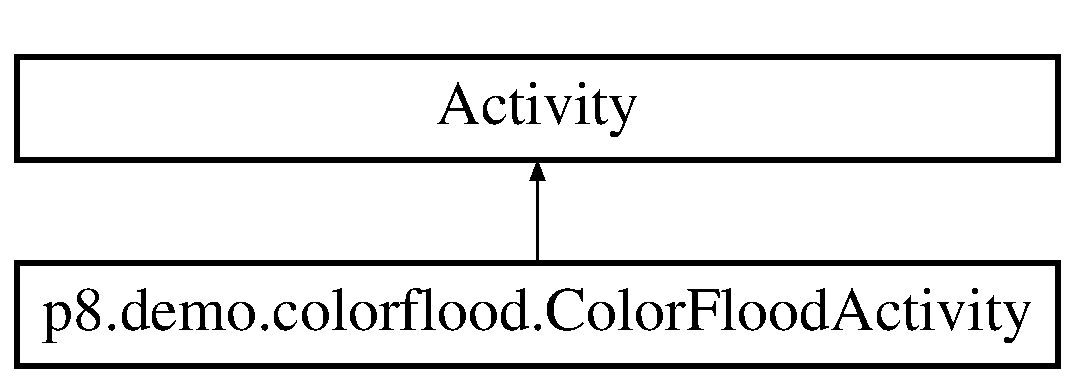
\includegraphics[height=2.000000cm]{classp8_1_1demo_1_1colorflood_1_1_color_flood_activity}
\end{center}
\end{figure}
\subsection*{Fonctions membres publiques}
\begin{DoxyCompactItemize}
\item 
void \hyperlink{classp8_1_1demo_1_1colorflood_1_1_color_flood_activity_a34e116c4a353266c0356fa19ff850307}{on\+Create} (Bundle saved\+Instance\+State)
\item 
void \hyperlink{classp8_1_1demo_1_1colorflood_1_1_color_flood_activity_af318bc90e1d129cc573184b92c4f1331}{on\+Pause} ()
\item 
void \hyperlink{classp8_1_1demo_1_1colorflood_1_1_color_flood_activity_ab94cb3fb2a0c95a3cf6eb2cde0535877}{on\+Resume} ()
\item 
void \hyperlink{classp8_1_1demo_1_1colorflood_1_1_color_flood_activity_a7c4b18f861611b81114183d34ed9bc4f}{on\+Stop} ()
\item 
void \hyperlink{classp8_1_1demo_1_1colorflood_1_1_color_flood_activity_a44048b3cc00c70ae3b49a1d925f06ac7}{on\+Restart} ()
\end{DoxyCompactItemize}


\subsection{Description détaillée}
la classe activité c\textquotesingle{}est la fenetre qui s\textquotesingle{}affiche sur le téléphone suite au declenchemeent de l\textquotesingle{}application ou l\textquotesingle{}interface graphique de l\textquotesingle{}application cette classe herite de la classe activité 

\subsection{Documentation des fonctions membres}
\hypertarget{classp8_1_1demo_1_1colorflood_1_1_color_flood_activity_a34e116c4a353266c0356fa19ff850307}{}\index{p8\+::demo\+::colorflood\+::\+Color\+Flood\+Activity@{p8\+::demo\+::colorflood\+::\+Color\+Flood\+Activity}!on\+Create@{on\+Create}}
\index{on\+Create@{on\+Create}!p8\+::demo\+::colorflood\+::\+Color\+Flood\+Activity@{p8\+::demo\+::colorflood\+::\+Color\+Flood\+Activity}}
\subsubsection[{on\+Create}]{\setlength{\rightskip}{0pt plus 5cm}void p8.\+demo.\+colorflood.\+Color\+Flood\+Activity.\+on\+Create (
\begin{DoxyParamCaption}
\item[{Bundle}]{saved\+Instance\+State}
\end{DoxyParamCaption}
)\hspace{0.3cm}{\ttfamily [inline]}}\label{classp8_1_1demo_1_1colorflood_1_1_color_flood_activity_a34e116c4a353266c0356fa19ff850307}
variable seekbar\+: correspond a la barre de progression

/$\ast$$\ast$ Cette méthode est la première qui est lancée au démarrage d\textquotesingle{}une application. 
\begin{DoxyParams}{Paramètres}
{\em saved\+Instance\+State} & quand l\textquotesingle{}application est rappelé après avoir tué par le système c\textquotesingle{}est a cela que sert le parametre de type Bundle \\
\hline
\end{DoxyParams}
on utilise cette methode pour forcer l\textquotesingle{}application a etre que en portrait et on peut pas tourner le telephone pour avoir le mode paysage 
\begin{DoxyParams}{Paramètres}
{\em Activity\+Info.\+S\+C\+R\+E\+E\+N\+\_\+\+O\+R\+I\+E\+N\+T\+A\+T\+I\+O\+N\+\_\+\+P\+O\+R\+T\+R\+A\+I\+T} & \\
\hline
\end{DoxyParams}
super.\+on\+Create\+: avec super on fait appel à une méthode ou un attribut qui appartient à la superclasse de la méthode actuelle. autrement dit a la classe activity

La méthode void set\+Content\+View (View vue) permet d\textquotesingle{}indiquer l\textquotesingle{}interface graphique de notre activité.

seek\+Bar = (Seek\+Bar) find\+View\+By\+Id(R.\+id.\+seek\+Bar)\+: on crée un objet de type seekbar ou barre de progression pour nos levels

seek\+Bar.\+set\+Max(4)\+: on défini le max de la barre a progression qui est égal a 4 c\textquotesingle{}est a dire de 0 a 4 ce qui correspond a nos 5 levels dans le jeu

la classe seek\+Bar.\+set\+On\+Seek\+Bar\+Change\+Listener c\textquotesingle{}est comme un rappel(callback) qui informe lorsque le niveau d\textquotesingle{}activité a été changé. cette classe elle contient 3 sous methode\+: on\+Progress\+Changed() on\+Start\+Tracking\+Touch() on\+Stop\+Tracking\+Touch()

int progress = 0\+: une variable progress qu\textquotesingle{}on l\textquotesingle{}initialise a 0 pour dire on commence toujours par le level 0

la methode on\+Progress\+Changed() elle sert quand la barre de progression elle change. 
\begin{DoxyParams}{Paramètres}
{\em seekbar} & c\textquotesingle{}est la barre dans laquelle on va effectuer le changement. \\
\hline
{\em progres\+Value} & la nouvelle valeur de la variable progress declaré la haut. \\
\hline
{\em Vrai} & si le changement d\textquotesingle{}étape a été lancée par l\textquotesingle{}utilisateur.\\
\hline
\end{DoxyParams}
la methode on\+Start\+Tracking\+Touch() elle permet d\textquotesingle{}avoir une Notification que l\textquotesingle{}utilisateur a commencé un geste tactile. 
\begin{DoxyParams}{Paramètres}
{\em seekbar} & c\textquotesingle{}est la barre dans laquelle on va effectuer le changement.\\
\hline
\end{DoxyParams}
la methode on\+Stop\+Tracking\+Touch() elle permet d\textquotesingle{}avoir une Notification que l\textquotesingle{}utilisateur a terminé un geste tactile. 
\begin{DoxyParams}{Paramètres}
{\em seekbar} & c\textquotesingle{}est la barre dans laquelle on va effectuer le changement.\\
\hline
\end{DoxyParams}
si l\textquotesingle{}etat est inferieur a 2 puissance le premier click de l\textquotesingle{}utilisateur alors on set le level selon la variable progress

on crée un objet view du meme type que la classe(\+Color\+Flood\+View) et ca va etre comme une reference a la vu qu\textquotesingle{}on a créé

set\+Visibility()\+: on peut masquer ou afficher des vues \hypertarget{classp8_1_1demo_1_1colorflood_1_1_color_flood_activity_af318bc90e1d129cc573184b92c4f1331}{}\index{p8\+::demo\+::colorflood\+::\+Color\+Flood\+Activity@{p8\+::demo\+::colorflood\+::\+Color\+Flood\+Activity}!on\+Pause@{on\+Pause}}
\index{on\+Pause@{on\+Pause}!p8\+::demo\+::colorflood\+::\+Color\+Flood\+Activity@{p8\+::demo\+::colorflood\+::\+Color\+Flood\+Activity}}
\subsubsection[{on\+Pause}]{\setlength{\rightskip}{0pt plus 5cm}void p8.\+demo.\+colorflood.\+Color\+Flood\+Activity.\+on\+Pause (
\begin{DoxyParamCaption}
{}
\end{DoxyParamCaption}
)\hspace{0.3cm}{\ttfamily [inline]}}\label{classp8_1_1demo_1_1colorflood_1_1_color_flood_activity_af318bc90e1d129cc573184b92c4f1331}
cete methode est appelé lorsque le système est sur le point de commencer à reprendre une activité précédente. super.\+on\+Pause()\+: avec super on fait appel à une méthode ou un attribut qui appartient à la superclasse de la méthode actuelle, dans ce cas c \textquotesingle{}est \hyperlink{classp8_1_1demo_1_1colorflood_1_1_color_flood_activity_af318bc90e1d129cc573184b92c4f1331}{on\+Pause()} \hypertarget{classp8_1_1demo_1_1colorflood_1_1_color_flood_activity_a44048b3cc00c70ae3b49a1d925f06ac7}{}\index{p8\+::demo\+::colorflood\+::\+Color\+Flood\+Activity@{p8\+::demo\+::colorflood\+::\+Color\+Flood\+Activity}!on\+Restart@{on\+Restart}}
\index{on\+Restart@{on\+Restart}!p8\+::demo\+::colorflood\+::\+Color\+Flood\+Activity@{p8\+::demo\+::colorflood\+::\+Color\+Flood\+Activity}}
\subsubsection[{on\+Restart}]{\setlength{\rightskip}{0pt plus 5cm}void p8.\+demo.\+colorflood.\+Color\+Flood\+Activity.\+on\+Restart (
\begin{DoxyParamCaption}
{}
\end{DoxyParamCaption}
)\hspace{0.3cm}{\ttfamily [inline]}}\label{classp8_1_1demo_1_1colorflood_1_1_color_flood_activity_a44048b3cc00c70ae3b49a1d925f06ac7}
cette methode est appelé après votre activité a été arrêté, avant d\textquotesingle{}être repris. view.\+set\+Restart(true)\+: a chaque fois cette methose est appelé on fait un restart a notre application

super.\+on\+Restart()\+: avec super on fait appel à une méthode ou un attribut qui appartient à la superclasse de la méthode actuelle, dans ce cas c \textquotesingle{}est \hyperlink{classp8_1_1demo_1_1colorflood_1_1_color_flood_activity_a44048b3cc00c70ae3b49a1d925f06ac7}{on\+Restart()} \hypertarget{classp8_1_1demo_1_1colorflood_1_1_color_flood_activity_ab94cb3fb2a0c95a3cf6eb2cde0535877}{}\index{p8\+::demo\+::colorflood\+::\+Color\+Flood\+Activity@{p8\+::demo\+::colorflood\+::\+Color\+Flood\+Activity}!on\+Resume@{on\+Resume}}
\index{on\+Resume@{on\+Resume}!p8\+::demo\+::colorflood\+::\+Color\+Flood\+Activity@{p8\+::demo\+::colorflood\+::\+Color\+Flood\+Activity}}
\subsubsection[{on\+Resume}]{\setlength{\rightskip}{0pt plus 5cm}void p8.\+demo.\+colorflood.\+Color\+Flood\+Activity.\+on\+Resume (
\begin{DoxyParamCaption}
{}
\end{DoxyParamCaption}
)\hspace{0.3cm}{\ttfamily [inline]}}\label{classp8_1_1demo_1_1colorflood_1_1_color_flood_activity_ab94cb3fb2a0c95a3cf6eb2cde0535877}
cette methode est appelé lorsque l\textquotesingle{}activité sera commencer à interagir avec l\textquotesingle{}utilisateur. super.\+on\+Resume()\+: avec super on fait appel à une méthode ou un attribut qui appartient à la superclasse de la méthode actuelle, dans ce cas c \textquotesingle{}est \hyperlink{classp8_1_1demo_1_1colorflood_1_1_color_flood_activity_ab94cb3fb2a0c95a3cf6eb2cde0535877}{on\+Resume()} \hypertarget{classp8_1_1demo_1_1colorflood_1_1_color_flood_activity_a7c4b18f861611b81114183d34ed9bc4f}{}\index{p8\+::demo\+::colorflood\+::\+Color\+Flood\+Activity@{p8\+::demo\+::colorflood\+::\+Color\+Flood\+Activity}!on\+Stop@{on\+Stop}}
\index{on\+Stop@{on\+Stop}!p8\+::demo\+::colorflood\+::\+Color\+Flood\+Activity@{p8\+::demo\+::colorflood\+::\+Color\+Flood\+Activity}}
\subsubsection[{on\+Stop}]{\setlength{\rightskip}{0pt plus 5cm}void p8.\+demo.\+colorflood.\+Color\+Flood\+Activity.\+on\+Stop (
\begin{DoxyParamCaption}
{}
\end{DoxyParamCaption}
)\hspace{0.3cm}{\ttfamily [inline]}}\label{classp8_1_1demo_1_1colorflood_1_1_color_flood_activity_a7c4b18f861611b81114183d34ed9bc4f}
cette methode est appelé lorsque l\textquotesingle{}activité est plus visible pour l\textquotesingle{}utilisateur, car une autre activité a été repris et couvrant celui-\/ci. super.\+on\+Stop()\+: avec super on fait appel à une méthode ou un attribut qui appartient à la superclasse de la méthode actuelle, dans ce cas c \textquotesingle{}est \hyperlink{classp8_1_1demo_1_1colorflood_1_1_color_flood_activity_a7c4b18f861611b81114183d34ed9bc4f}{on\+Stop()} 

La documentation de cette classe a été générée à partir du fichier suivant \+:\begin{DoxyCompactItemize}
\item 
\hyperlink{_color_flood_activity_8java}{Color\+Flood\+Activity.\+java}\end{DoxyCompactItemize}

\hypertarget{classp8_1_1demo_1_1colorflood_1_1_color_flood_view}{}\section{Référence de la classe p8.\+demo.\+colorflood.\+Color\+Flood\+View}
\label{classp8_1_1demo_1_1colorflood_1_1_color_flood_view}\index{p8.\+demo.\+colorflood.\+Color\+Flood\+View@{p8.\+demo.\+colorflood.\+Color\+Flood\+View}}
Graphe d\textquotesingle{}héritage de p8.\+demo.\+colorflood.\+Color\+Flood\+View\+:\begin{figure}[H]
\begin{center}
\leavevmode
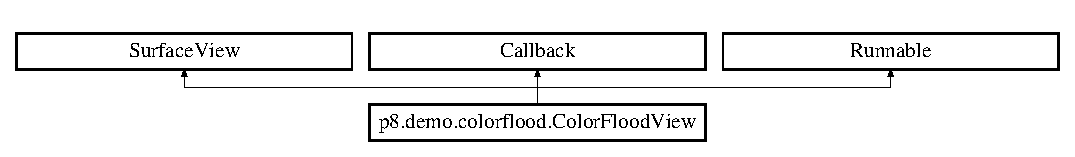
\includegraphics[height=1.666667cm]{classp8_1_1demo_1_1colorflood_1_1_color_flood_view}
\end{center}
\end{figure}
\subsection*{Fonctions membres publiques}
\begin{DoxyCompactItemize}
\item 
\hypertarget{classp8_1_1demo_1_1colorflood_1_1_color_flood_view_a28d78e47c2619a9d2791ea379ef059b2}{}{\bfseries Color\+Flood\+View} (Context context, Attribute\+Set attrs)\label{classp8_1_1demo_1_1colorflood_1_1_color_flood_view_a28d78e47c2619a9d2791ea379ef059b2}

\item 
void \hyperlink{classp8_1_1demo_1_1colorflood_1_1_color_flood_view_ac9757650005dc20325dd80e17b58c55a}{initparameters} ()
\item 
void \hyperlink{classp8_1_1demo_1_1colorflood_1_1_color_flood_view_a208f67a9f808f3dc8f683eb566810884}{init\+Max} ()
\item 
void \hyperlink{classp8_1_1demo_1_1colorflood_1_1_color_flood_view_af904e361cda2271b0ebf7c10963d0edc}{set\+Level} (int level)
\item 
void \hyperlink{classp8_1_1demo_1_1colorflood_1_1_color_flood_view_a3886613e29f4a823d6d8bcc0f2393b85}{set\+Restart} (boolean restart)
\item 
boolean \hyperlink{classp8_1_1demo_1_1colorflood_1_1_color_flood_view_a1fe95dbfaf8bfe98e49b2d8b688085c1}{get\+First\+Click} ()
\item 
void \hyperlink{classp8_1_1demo_1_1colorflood_1_1_color_flood_view_a0965d8ffa4f137a28f4bf22bd4ac6a2a}{paint\+Choice} (Canvas canvas)
\item 
void \hyperlink{classp8_1_1demo_1_1colorflood_1_1_color_flood_view_aa989675b60f6fcbbe3a4c9a7be4b1561}{paint\+Score} (Canvas canvas)
\item 
void \hyperlink{classp8_1_1demo_1_1colorflood_1_1_color_flood_view_ac3a53a838779e02bc3629e4a49676fd2}{paint\+Highscore} (Canvas canvas)
\item 
int \hyperlink{classp8_1_1demo_1_1colorflood_1_1_color_flood_view_a5666b3002546f071f8e503c009608259}{state} ()
\item 
int \hyperlink{classp8_1_1demo_1_1colorflood_1_1_color_flood_view_a9ca13be0b3ba4f0555ebf44a31634353}{get\+Highscore} ()
\item 
void \hyperlink{classp8_1_1demo_1_1colorflood_1_1_color_flood_view_a8b5270516723415941e281fd45f66093}{save\+Score} ()
\item 
\hypertarget{classp8_1_1demo_1_1colorflood_1_1_color_flood_view_ad14c5593f1ffa3b9693d2498ad9b9ae7}{}void {\bfseries surface\+Changed} (Surface\+Holder holder, int format, int width, int height)\label{classp8_1_1demo_1_1colorflood_1_1_color_flood_view_ad14c5593f1ffa3b9693d2498ad9b9ae7}

\item 
\hypertarget{classp8_1_1demo_1_1colorflood_1_1_color_flood_view_a2d67d0a5b8d4bb83b698e517f3883d53}{}void {\bfseries surface\+Created} (Surface\+Holder arg0)\label{classp8_1_1demo_1_1colorflood_1_1_color_flood_view_a2d67d0a5b8d4bb83b698e517f3883d53}

\item 
\hypertarget{classp8_1_1demo_1_1colorflood_1_1_color_flood_view_a21bd9618fd8febc1ac9218afb61e8cf9}{}void {\bfseries surface\+Destroyed} (Surface\+Holder arg0)\label{classp8_1_1demo_1_1colorflood_1_1_color_flood_view_a21bd9618fd8febc1ac9218afb61e8cf9}

\item 
void \hyperlink{classp8_1_1demo_1_1colorflood_1_1_color_flood_view_ac36fac9e9c09e4ce941f34dc5e88a339}{run} ()
\item 
void \hyperlink{classp8_1_1demo_1_1colorflood_1_1_color_flood_view_a816914982568d39c00fd585b57df2d26}{test\+Voisin} (int x, int y)
\item 
void \hyperlink{classp8_1_1demo_1_1colorflood_1_1_color_flood_view_a6ec591cc35c1d2d3b58376f7ab843adf}{change\+Color} (int color)
\item 
void \hyperlink{classp8_1_1demo_1_1colorflood_1_1_color_flood_view_ac4be93ac702ce5142f93b4670e1e0e60}{click\+Circle} (int color)
\item 
boolean \hyperlink{classp8_1_1demo_1_1colorflood_1_1_color_flood_view_a033731c2d315d3aecadc578fa2648438}{on\+Touch\+Event} (Motion\+Event event)
\item 
Parcelable \hyperlink{classp8_1_1demo_1_1colorflood_1_1_color_flood_view_a77325bff94dd30de94b10af41846ca03}{on\+Save\+Instance\+State} ()
\item 
void \hyperlink{classp8_1_1demo_1_1colorflood_1_1_color_flood_view_a1b4e4c683f66ab8bf16f72453b8c8ff0}{on\+Restore\+Instance\+State} (Parcelable \hyperlink{classp8_1_1demo_1_1colorflood_1_1_color_flood_view_a5666b3002546f071f8e503c009608259}{state})
\end{DoxyCompactItemize}
\subsection*{Attributs publics statiques}
\begin{DoxyCompactItemize}
\item 
static final String \hyperlink{classp8_1_1demo_1_1colorflood_1_1_color_flood_view_a4d0c7b140ad6fef18d29c6fc088b6471}{P\+R\+E\+F\+S\+\_\+\+N\+A\+M\+E} = \char`\"{}My\+Prefs\+File\char`\"{}
\end{DoxyCompactItemize}


\subsection{Description détaillée}
la classe \hyperlink{classp8_1_1demo_1_1colorflood_1_1_color_flood_view}{Color\+Flood\+View} c\textquotesingle{}est la classe principale de notre jeu elle contient tout les element necessaire pour developper le jeu elle herite de la classe surface\+View et implemente des classes callback et Runnable pour le thread utilisé 

\subsection{Documentation des fonctions membres}
\hypertarget{classp8_1_1demo_1_1colorflood_1_1_color_flood_view_a6ec591cc35c1d2d3b58376f7ab843adf}{}\index{p8\+::demo\+::colorflood\+::\+Color\+Flood\+View@{p8\+::demo\+::colorflood\+::\+Color\+Flood\+View}!change\+Color@{change\+Color}}
\index{change\+Color@{change\+Color}!p8\+::demo\+::colorflood\+::\+Color\+Flood\+View@{p8\+::demo\+::colorflood\+::\+Color\+Flood\+View}}
\subsubsection[{change\+Color}]{\setlength{\rightskip}{0pt plus 5cm}void p8.\+demo.\+colorflood.\+Color\+Flood\+View.\+change\+Color (
\begin{DoxyParamCaption}
\item[{int}]{color}
\end{DoxyParamCaption}
)\hspace{0.3cm}{\ttfamily [inline]}}\label{classp8_1_1demo_1_1colorflood_1_1_color_flood_view_a6ec591cc35c1d2d3b58376f7ab843adf}
A utiliser après la méthode test\+Voisin Change la couleur des cases dont la case vaut 10 par la couleur passée en paramètre 
\begin{DoxyParams}{Paramètres}
{\em color} & code de la couleur dont on souhaite colorier \\
\hline
\end{DoxyParams}
\hypertarget{classp8_1_1demo_1_1colorflood_1_1_color_flood_view_ac4be93ac702ce5142f93b4670e1e0e60}{}\index{p8\+::demo\+::colorflood\+::\+Color\+Flood\+View@{p8\+::demo\+::colorflood\+::\+Color\+Flood\+View}!click\+Circle@{click\+Circle}}
\index{click\+Circle@{click\+Circle}!p8\+::demo\+::colorflood\+::\+Color\+Flood\+View@{p8\+::demo\+::colorflood\+::\+Color\+Flood\+View}}
\subsubsection[{click\+Circle}]{\setlength{\rightskip}{0pt plus 5cm}void p8.\+demo.\+colorflood.\+Color\+Flood\+View.\+click\+Circle (
\begin{DoxyParamCaption}
\item[{int}]{color}
\end{DoxyParamCaption}
)\hspace{0.3cm}{\ttfamily [inline]}}\label{classp8_1_1demo_1_1colorflood_1_1_color_flood_view_ac4be93ac702ce5142f93b4670e1e0e60}
Gestion des interactions avec les cercles de couleur 
\begin{DoxyParams}{Paramètres}
{\em color} & \\
\hline
\end{DoxyParams}
\hypertarget{classp8_1_1demo_1_1colorflood_1_1_color_flood_view_a1fe95dbfaf8bfe98e49b2d8b688085c1}{}\index{p8\+::demo\+::colorflood\+::\+Color\+Flood\+View@{p8\+::demo\+::colorflood\+::\+Color\+Flood\+View}!get\+First\+Click@{get\+First\+Click}}
\index{get\+First\+Click@{get\+First\+Click}!p8\+::demo\+::colorflood\+::\+Color\+Flood\+View@{p8\+::demo\+::colorflood\+::\+Color\+Flood\+View}}
\subsubsection[{get\+First\+Click}]{\setlength{\rightskip}{0pt plus 5cm}boolean p8.\+demo.\+colorflood.\+Color\+Flood\+View.\+get\+First\+Click (
\begin{DoxyParamCaption}
{}
\end{DoxyParamCaption}
)\hspace{0.3cm}{\ttfamily [inline]}}\label{classp8_1_1demo_1_1colorflood_1_1_color_flood_view_a1fe95dbfaf8bfe98e49b2d8b688085c1}
retourne le premier click de l\textquotesingle{}utilisateur \hypertarget{classp8_1_1demo_1_1colorflood_1_1_color_flood_view_a9ca13be0b3ba4f0555ebf44a31634353}{}\index{p8\+::demo\+::colorflood\+::\+Color\+Flood\+View@{p8\+::demo\+::colorflood\+::\+Color\+Flood\+View}!get\+Highscore@{get\+Highscore}}
\index{get\+Highscore@{get\+Highscore}!p8\+::demo\+::colorflood\+::\+Color\+Flood\+View@{p8\+::demo\+::colorflood\+::\+Color\+Flood\+View}}
\subsubsection[{get\+Highscore}]{\setlength{\rightskip}{0pt plus 5cm}int p8.\+demo.\+colorflood.\+Color\+Flood\+View.\+get\+Highscore (
\begin{DoxyParamCaption}
{}
\end{DoxyParamCaption}
)\hspace{0.3cm}{\ttfamily [inline]}}\label{classp8_1_1demo_1_1colorflood_1_1_color_flood_view_a9ca13be0b3ba4f0555ebf44a31634353}
Récupère le meilleur score pour le niveau courant (par défaut le score maximum où l\textquotesingle{}on peut gagner) \begin{DoxyReturn}{Renvoie}
meilleure score du niveau 
\end{DoxyReturn}
\hypertarget{classp8_1_1demo_1_1colorflood_1_1_color_flood_view_a208f67a9f808f3dc8f683eb566810884}{}\index{p8\+::demo\+::colorflood\+::\+Color\+Flood\+View@{p8\+::demo\+::colorflood\+::\+Color\+Flood\+View}!init\+Max@{init\+Max}}
\index{init\+Max@{init\+Max}!p8\+::demo\+::colorflood\+::\+Color\+Flood\+View@{p8\+::demo\+::colorflood\+::\+Color\+Flood\+View}}
\subsubsection[{init\+Max}]{\setlength{\rightskip}{0pt plus 5cm}void p8.\+demo.\+colorflood.\+Color\+Flood\+View.\+init\+Max (
\begin{DoxyParamCaption}
{}
\end{DoxyParamCaption}
)\hspace{0.3cm}{\ttfamily [inline]}}\label{classp8_1_1demo_1_1colorflood_1_1_color_flood_view_a208f67a9f808f3dc8f683eb566810884}
Détermine le score maximum pour gagner pour chaque niveau \hypertarget{classp8_1_1demo_1_1colorflood_1_1_color_flood_view_ac9757650005dc20325dd80e17b58c55a}{}\index{p8\+::demo\+::colorflood\+::\+Color\+Flood\+View@{p8\+::demo\+::colorflood\+::\+Color\+Flood\+View}!initparameters@{initparameters}}
\index{initparameters@{initparameters}!p8\+::demo\+::colorflood\+::\+Color\+Flood\+View@{p8\+::demo\+::colorflood\+::\+Color\+Flood\+View}}
\subsubsection[{initparameters}]{\setlength{\rightskip}{0pt plus 5cm}void p8.\+demo.\+colorflood.\+Color\+Flood\+View.\+initparameters (
\begin{DoxyParamCaption}
{}
\end{DoxyParamCaption}
)\hspace{0.3cm}{\ttfamily [inline]}}\label{classp8_1_1demo_1_1colorflood_1_1_color_flood_view_ac9757650005dc20325dd80e17b58c55a}
initialiser les parametre de notre jeu \hypertarget{classp8_1_1demo_1_1colorflood_1_1_color_flood_view_a1b4e4c683f66ab8bf16f72453b8c8ff0}{}\index{p8\+::demo\+::colorflood\+::\+Color\+Flood\+View@{p8\+::demo\+::colorflood\+::\+Color\+Flood\+View}!on\+Restore\+Instance\+State@{on\+Restore\+Instance\+State}}
\index{on\+Restore\+Instance\+State@{on\+Restore\+Instance\+State}!p8\+::demo\+::colorflood\+::\+Color\+Flood\+View@{p8\+::demo\+::colorflood\+::\+Color\+Flood\+View}}
\subsubsection[{on\+Restore\+Instance\+State}]{\setlength{\rightskip}{0pt plus 5cm}void p8.\+demo.\+colorflood.\+Color\+Flood\+View.\+on\+Restore\+Instance\+State (
\begin{DoxyParamCaption}
\item[{Parcelable}]{state}
\end{DoxyParamCaption}
)\hspace{0.3cm}{\ttfamily [inline]}}\label{classp8_1_1demo_1_1colorflood_1_1_color_flood_view_a1b4e4c683f66ab8bf16f72453b8c8ff0}
Charge l\textquotesingle{}état de la vue précedemment sauvergardée 
\begin{DoxyParams}{Paramètres}
{\em state} & \\
\hline
\end{DoxyParams}
\hypertarget{classp8_1_1demo_1_1colorflood_1_1_color_flood_view_a77325bff94dd30de94b10af41846ca03}{}\index{p8\+::demo\+::colorflood\+::\+Color\+Flood\+View@{p8\+::demo\+::colorflood\+::\+Color\+Flood\+View}!on\+Save\+Instance\+State@{on\+Save\+Instance\+State}}
\index{on\+Save\+Instance\+State@{on\+Save\+Instance\+State}!p8\+::demo\+::colorflood\+::\+Color\+Flood\+View@{p8\+::demo\+::colorflood\+::\+Color\+Flood\+View}}
\subsubsection[{on\+Save\+Instance\+State}]{\setlength{\rightskip}{0pt plus 5cm}Parcelable p8.\+demo.\+colorflood.\+Color\+Flood\+View.\+on\+Save\+Instance\+State (
\begin{DoxyParamCaption}
{}
\end{DoxyParamCaption}
)\hspace{0.3cm}{\ttfamily [inline]}}\label{classp8_1_1demo_1_1colorflood_1_1_color_flood_view_a77325bff94dd30de94b10af41846ca03}
Sauvegarde l\textquotesingle{}état de la vue \begin{DoxyReturn}{Renvoie}

\end{DoxyReturn}
\hypertarget{classp8_1_1demo_1_1colorflood_1_1_color_flood_view_a033731c2d315d3aecadc578fa2648438}{}\index{p8\+::demo\+::colorflood\+::\+Color\+Flood\+View@{p8\+::demo\+::colorflood\+::\+Color\+Flood\+View}!on\+Touch\+Event@{on\+Touch\+Event}}
\index{on\+Touch\+Event@{on\+Touch\+Event}!p8\+::demo\+::colorflood\+::\+Color\+Flood\+View@{p8\+::demo\+::colorflood\+::\+Color\+Flood\+View}}
\subsubsection[{on\+Touch\+Event}]{\setlength{\rightskip}{0pt plus 5cm}boolean p8.\+demo.\+colorflood.\+Color\+Flood\+View.\+on\+Touch\+Event (
\begin{DoxyParamCaption}
\item[{Motion\+Event}]{event}
\end{DoxyParamCaption}
)\hspace{0.3cm}{\ttfamily [inline]}}\label{classp8_1_1demo_1_1colorflood_1_1_color_flood_view_a033731c2d315d3aecadc578fa2648438}
Gestion des évènements tactiles 
\begin{DoxyParams}{Paramètres}
{\em event} & \\
\hline
\end{DoxyParams}
\begin{DoxyReturn}{Renvoie}

\end{DoxyReturn}
\hypertarget{classp8_1_1demo_1_1colorflood_1_1_color_flood_view_a0965d8ffa4f137a28f4bf22bd4ac6a2a}{}\index{p8\+::demo\+::colorflood\+::\+Color\+Flood\+View@{p8\+::demo\+::colorflood\+::\+Color\+Flood\+View}!paint\+Choice@{paint\+Choice}}
\index{paint\+Choice@{paint\+Choice}!p8\+::demo\+::colorflood\+::\+Color\+Flood\+View@{p8\+::demo\+::colorflood\+::\+Color\+Flood\+View}}
\subsubsection[{paint\+Choice}]{\setlength{\rightskip}{0pt plus 5cm}void p8.\+demo.\+colorflood.\+Color\+Flood\+View.\+paint\+Choice (
\begin{DoxyParamCaption}
\item[{Canvas}]{canvas}
\end{DoxyParamCaption}
)\hspace{0.3cm}{\ttfamily [inline]}}\label{classp8_1_1demo_1_1colorflood_1_1_color_flood_view_a0965d8ffa4f137a28f4bf22bd4ac6a2a}
Dessine les cercles de couleurs en-\/dessous du plateau, avec lesquels l\textquotesingle{}utilisateur peut interagir 
\begin{DoxyParams}{Paramètres}
{\em canvas} & \\
\hline
\end{DoxyParams}
\hypertarget{classp8_1_1demo_1_1colorflood_1_1_color_flood_view_ac3a53a838779e02bc3629e4a49676fd2}{}\index{p8\+::demo\+::colorflood\+::\+Color\+Flood\+View@{p8\+::demo\+::colorflood\+::\+Color\+Flood\+View}!paint\+Highscore@{paint\+Highscore}}
\index{paint\+Highscore@{paint\+Highscore}!p8\+::demo\+::colorflood\+::\+Color\+Flood\+View@{p8\+::demo\+::colorflood\+::\+Color\+Flood\+View}}
\subsubsection[{paint\+Highscore}]{\setlength{\rightskip}{0pt plus 5cm}void p8.\+demo.\+colorflood.\+Color\+Flood\+View.\+paint\+Highscore (
\begin{DoxyParamCaption}
\item[{Canvas}]{canvas}
\end{DoxyParamCaption}
)\hspace{0.3cm}{\ttfamily [inline]}}\label{classp8_1_1demo_1_1colorflood_1_1_color_flood_view_ac3a53a838779e02bc3629e4a49676fd2}
Dessine le meilleur score du niveau 
\begin{DoxyParams}{Paramètres}
{\em canvas} & \\
\hline
\end{DoxyParams}
\hypertarget{classp8_1_1demo_1_1colorflood_1_1_color_flood_view_aa989675b60f6fcbbe3a4c9a7be4b1561}{}\index{p8\+::demo\+::colorflood\+::\+Color\+Flood\+View@{p8\+::demo\+::colorflood\+::\+Color\+Flood\+View}!paint\+Score@{paint\+Score}}
\index{paint\+Score@{paint\+Score}!p8\+::demo\+::colorflood\+::\+Color\+Flood\+View@{p8\+::demo\+::colorflood\+::\+Color\+Flood\+View}}
\subsubsection[{paint\+Score}]{\setlength{\rightskip}{0pt plus 5cm}void p8.\+demo.\+colorflood.\+Color\+Flood\+View.\+paint\+Score (
\begin{DoxyParamCaption}
\item[{Canvas}]{canvas}
\end{DoxyParamCaption}
)\hspace{0.3cm}{\ttfamily [inline]}}\label{classp8_1_1demo_1_1colorflood_1_1_color_flood_view_aa989675b60f6fcbbe3a4c9a7be4b1561}
Dessine le score actuel au-\/dessus du plateau de jeu 
\begin{DoxyParams}{Paramètres}
{\em canvas} & \\
\hline
\end{DoxyParams}
\hypertarget{classp8_1_1demo_1_1colorflood_1_1_color_flood_view_ac36fac9e9c09e4ce941f34dc5e88a339}{}\index{p8\+::demo\+::colorflood\+::\+Color\+Flood\+View@{p8\+::demo\+::colorflood\+::\+Color\+Flood\+View}!run@{run}}
\index{run@{run}!p8\+::demo\+::colorflood\+::\+Color\+Flood\+View@{p8\+::demo\+::colorflood\+::\+Color\+Flood\+View}}
\subsubsection[{run}]{\setlength{\rightskip}{0pt plus 5cm}void p8.\+demo.\+colorflood.\+Color\+Flood\+View.\+run (
\begin{DoxyParamCaption}
{}
\end{DoxyParamCaption}
)\hspace{0.3cm}{\ttfamily [inline]}}\label{classp8_1_1demo_1_1colorflood_1_1_color_flood_view_ac36fac9e9c09e4ce941f34dc5e88a339}
On endort le thread, modifie le compteur d\textquotesingle{}animation, on bloque le canvas, on dessine puis on libère le canvas \hypertarget{classp8_1_1demo_1_1colorflood_1_1_color_flood_view_a8b5270516723415941e281fd45f66093}{}\index{p8\+::demo\+::colorflood\+::\+Color\+Flood\+View@{p8\+::demo\+::colorflood\+::\+Color\+Flood\+View}!save\+Score@{save\+Score}}
\index{save\+Score@{save\+Score}!p8\+::demo\+::colorflood\+::\+Color\+Flood\+View@{p8\+::demo\+::colorflood\+::\+Color\+Flood\+View}}
\subsubsection[{save\+Score}]{\setlength{\rightskip}{0pt plus 5cm}void p8.\+demo.\+colorflood.\+Color\+Flood\+View.\+save\+Score (
\begin{DoxyParamCaption}
{}
\end{DoxyParamCaption}
)\hspace{0.3cm}{\ttfamily [inline]}}\label{classp8_1_1demo_1_1colorflood_1_1_color_flood_view_a8b5270516723415941e281fd45f66093}
Sauvegarde le score pour le niveau courant \hypertarget{classp8_1_1demo_1_1colorflood_1_1_color_flood_view_af904e361cda2271b0ebf7c10963d0edc}{}\index{p8\+::demo\+::colorflood\+::\+Color\+Flood\+View@{p8\+::demo\+::colorflood\+::\+Color\+Flood\+View}!set\+Level@{set\+Level}}
\index{set\+Level@{set\+Level}!p8\+::demo\+::colorflood\+::\+Color\+Flood\+View@{p8\+::demo\+::colorflood\+::\+Color\+Flood\+View}}
\subsubsection[{set\+Level}]{\setlength{\rightskip}{0pt plus 5cm}void p8.\+demo.\+colorflood.\+Color\+Flood\+View.\+set\+Level (
\begin{DoxyParamCaption}
\item[{int}]{level}
\end{DoxyParamCaption}
)\hspace{0.3cm}{\ttfamily [inline]}}\label{classp8_1_1demo_1_1colorflood_1_1_color_flood_view_af904e361cda2271b0ebf7c10963d0edc}
Détermine le niveau voulu et initialise les paramètres et le plateau en conséquence 
\begin{DoxyParams}{Paramètres}
{\em level} & numéro de niveau sélectionné dans la Seek\+Bar \\
\hline
\end{DoxyParams}
\hypertarget{classp8_1_1demo_1_1colorflood_1_1_color_flood_view_a3886613e29f4a823d6d8bcc0f2393b85}{}\index{p8\+::demo\+::colorflood\+::\+Color\+Flood\+View@{p8\+::demo\+::colorflood\+::\+Color\+Flood\+View}!set\+Restart@{set\+Restart}}
\index{set\+Restart@{set\+Restart}!p8\+::demo\+::colorflood\+::\+Color\+Flood\+View@{p8\+::demo\+::colorflood\+::\+Color\+Flood\+View}}
\subsubsection[{set\+Restart}]{\setlength{\rightskip}{0pt plus 5cm}void p8.\+demo.\+colorflood.\+Color\+Flood\+View.\+set\+Restart (
\begin{DoxyParamCaption}
\item[{boolean}]{restart}
\end{DoxyParamCaption}
)\hspace{0.3cm}{\ttfamily [inline]}}\label{classp8_1_1demo_1_1colorflood_1_1_color_flood_view_a3886613e29f4a823d6d8bcc0f2393b85}
quand l\textquotesingle{}application redemarre 
\begin{DoxyParams}{Paramètres}
{\em restart} & c\textquotesingle{}est un booleen qui nous dit si l\textquotesingle{}appli est redemarré ou non \\
\hline
\end{DoxyParams}
\hypertarget{classp8_1_1demo_1_1colorflood_1_1_color_flood_view_a5666b3002546f071f8e503c009608259}{}\index{p8\+::demo\+::colorflood\+::\+Color\+Flood\+View@{p8\+::demo\+::colorflood\+::\+Color\+Flood\+View}!state@{state}}
\index{state@{state}!p8\+::demo\+::colorflood\+::\+Color\+Flood\+View@{p8\+::demo\+::colorflood\+::\+Color\+Flood\+View}}
\subsubsection[{state}]{\setlength{\rightskip}{0pt plus 5cm}int p8.\+demo.\+colorflood.\+Color\+Flood\+View.\+state (
\begin{DoxyParamCaption}
{}
\end{DoxyParamCaption}
)\hspace{0.3cm}{\ttfamily [inline]}}\label{classp8_1_1demo_1_1colorflood_1_1_color_flood_view_a5666b3002546f071f8e503c009608259}
Retourne l\textquotesingle{}état actuel du jeu (gagné, perdu, peut encore jouer) \begin{DoxyReturn}{Renvoie}
0\+:gagné, 1\+:perdu, 2\+:peut continuer à jouer 
\end{DoxyReturn}
\hypertarget{classp8_1_1demo_1_1colorflood_1_1_color_flood_view_a816914982568d39c00fd585b57df2d26}{}\index{p8\+::demo\+::colorflood\+::\+Color\+Flood\+View@{p8\+::demo\+::colorflood\+::\+Color\+Flood\+View}!test\+Voisin@{test\+Voisin}}
\index{test\+Voisin@{test\+Voisin}!p8\+::demo\+::colorflood\+::\+Color\+Flood\+View@{p8\+::demo\+::colorflood\+::\+Color\+Flood\+View}}
\subsubsection[{test\+Voisin}]{\setlength{\rightskip}{0pt plus 5cm}void p8.\+demo.\+colorflood.\+Color\+Flood\+View.\+test\+Voisin (
\begin{DoxyParamCaption}
\item[{int}]{x, }
\item[{int}]{y}
\end{DoxyParamCaption}
)\hspace{0.3cm}{\ttfamily [inline]}}\label{classp8_1_1demo_1_1colorflood_1_1_color_flood_view_a816914982568d39c00fd585b57df2d26}
Fonction récursive qui va tester la couleur de chaque voisin et mettre à 10 les cases répondant aux critères 
\begin{DoxyParams}{Paramètres}
{\em x} & position en x de la case à tester \\
\hline
{\em y} & position en y de la case à tester \\
\hline
\end{DoxyParams}


\subsection{Documentation des données membres}
\hypertarget{classp8_1_1demo_1_1colorflood_1_1_color_flood_view_a4d0c7b140ad6fef18d29c6fc088b6471}{}\index{p8\+::demo\+::colorflood\+::\+Color\+Flood\+View@{p8\+::demo\+::colorflood\+::\+Color\+Flood\+View}!P\+R\+E\+F\+S\+\_\+\+N\+A\+M\+E@{P\+R\+E\+F\+S\+\_\+\+N\+A\+M\+E}}
\index{P\+R\+E\+F\+S\+\_\+\+N\+A\+M\+E@{P\+R\+E\+F\+S\+\_\+\+N\+A\+M\+E}!p8\+::demo\+::colorflood\+::\+Color\+Flood\+View@{p8\+::demo\+::colorflood\+::\+Color\+Flood\+View}}
\subsubsection[{P\+R\+E\+F\+S\+\_\+\+N\+A\+M\+E}]{\setlength{\rightskip}{0pt plus 5cm}final String p8.\+demo.\+colorflood.\+Color\+Flood\+View.\+P\+R\+E\+F\+S\+\_\+\+N\+A\+M\+E = \char`\"{}My\+Prefs\+File\char`\"{}\hspace{0.3cm}{\ttfamily [static]}}\label{classp8_1_1demo_1_1colorflood_1_1_color_flood_view_a4d0c7b140ad6fef18d29c6fc088b6471}
utilisé pour la sauvegarde du meilleur score 

La documentation de cette classe a été générée à partir du fichier suivant \+:\begin{DoxyCompactItemize}
\item 
\hyperlink{_color_flood_view_8java}{Color\+Flood\+View.\+java}\end{DoxyCompactItemize}

\chapter{Documentation des fichiers}
\hypertarget{_color_flood_activity_8java}{}\section{Référence du fichier Color\+Flood\+Activity.\+java}
\label{_color_flood_activity_8java}\index{Color\+Flood\+Activity.\+java@{Color\+Flood\+Activity.\+java}}


ce code représente notre projet de developpement android qui consiste a faire un jeu \char`\"{}color Flood\char`\"{} sous android (celui ci est l\textquotesingle{}activité de notre application)  


\subsection*{Classes}
\begin{DoxyCompactItemize}
\item 
class \hyperlink{classp8_1_1demo_1_1colorflood_1_1_color_flood_activity}{p8.\+demo.\+colorflood.\+Color\+Flood\+Activity}
\end{DoxyCompactItemize}


\subsection{Description détaillée}
ce code représente notre projet de developpement android qui consiste a faire un jeu \char`\"{}color Flood\char`\"{} sous android (celui ci est l\textquotesingle{}activité de notre application) 

\begin{DoxyAuthor}{Auteur}
L\+E\+C\+O\+C\+Q Guillaume F\+O\+U\+Z\+R\+I Wael 
\end{DoxyAuthor}

\hypertarget{_color_flood_view_8java}{}\section{Référence du fichier Color\+Flood\+View.\+java}
\label{_color_flood_view_8java}\index{Color\+Flood\+View.\+java@{Color\+Flood\+View.\+java}}


ce code représente notre projet de developpement android qui consiste a faire un jeu \char`\"{}color Flood\char`\"{} sous android (celui ci est la \char`\"{}\+View\char`\"{} de notre application)  


\subsection*{Classes}
\begin{DoxyCompactItemize}
\item 
class \hyperlink{classp8_1_1demo_1_1colorflood_1_1_color_flood_view}{p8.\+demo.\+colorflood.\+Color\+Flood\+View}
\end{DoxyCompactItemize}


\subsection{Description détaillée}
ce code représente notre projet de developpement android qui consiste a faire un jeu \char`\"{}color Flood\char`\"{} sous android (celui ci est la \char`\"{}\+View\char`\"{} de notre application) 

\begin{DoxyAuthor}{Auteur}
L\+E\+C\+O\+C\+Q Guillaume F\+O\+U\+Z\+R\+I Wael 
\end{DoxyAuthor}

%--- End generated contents ---

% Index
\backmatter
\newpage
\phantomsection
\clearemptydoublepage
\addcontentsline{toc}{chapter}{Index}
\printindex

\end{document}
